% L15a figure: what the explicit Euler method does, for one state variable.
%
%   (a) One step from the exact state. The model is dx/dt = 1 - x, with
%       x(t_k) = 0.2 and a step of 0.9 time units. The Euler step follows the
%       tangent, with slope f = 1 - 0.2 = 0.8, to 0.2 + 0.9(0.8) = 0.92. The
%       exact state is x(t_{k+1}) = 1 - 0.8 exp(-0.9) = 0.6747. The gap
%       between the two points is the local error.
%   (b) Three steps from x_0 = 0.05 on the logistic model dx/dt = x(1 - x),
%       with a step of 1.2 time units. The computed states are 0.107, 0.2217,
%       and 0.4287. The exact solution is x(t) = 1/(1 + 19 exp(-t)), with
%       x(t_3) = 0.6583. Each gray curve is the exact solution through a
%       computed state, 1/(1 + C exp(-(t - t_j))) with C = 1/x_j - 1
%       (C = 8.3458 at t_1 and C = 3.5114 at t_2).
%
% Panel (b) uses the logistic model because the gaps between its solution
% curves at t_3 stay wide enough to show both gray curves; the solution curves
% of the model in (a) bunch together.
%
% Layout: every panel in this figure and in Fig-RungeKutta-Stages has the same
% axis box, 7.94 cm wide and 5.18 cm tall, with its lower-left corner on the
% baseline. Panel (a) uses the scale and the step of both panels of
% Fig-RungeKutta-Stages (5.4 cm per unit on both axes), so the three single
% steps can be compared side by side.
%
% Drawn on November 27, 2026 with the palette and build of the L14a figures.
% The notebook SVG carries a dark palette added by theme_svg.py; keep new colors
% in that script's mapping when changing the palette here.
\documentclass[tikz,border=4pt]{standalone}
\usepackage{amsmath}
\usepackage[no-math]{fontspec}
\IfFontExistsTF{Arial}{\setsansfont{Arial}}{\setsansfont{TeX Gyre Heros}}
\renewcommand{\familydefault}{\sfdefault}
\usetikzlibrary{arrows.meta, decorations.pathreplacing}

% Ink, blue, red, and gray match the L14a and L13a figures. Blue draws the exact
% solution, red draws what the method computes, and gray draws the guides and
% the exact solutions through the computed states.
\definecolor{vnink}{HTML}{202124}
\definecolor{gdblue}{HTML}{0091FF}
\definecolor{evred}{HTML}{D93025}
\definecolor{gdgray}{HTML}{6D7278}

\newcommand{\vx}{\mathbf{x}}
\newcommand{\hx}{\hat{\mathbf{x}}}

\tikzset{
  axis/.style={draw=vnink, line width=0.6pt, -{Stealth[length=2mm, width=1.6mm]}},
  tick/.style={draw=vnink, line width=0.6pt},
  ticklab/.style={text=vnink, font=\small, anchor=north},
  axlab/.style={text=vnink, font=\sffamily\small},
  exact/.style={draw=gdblue, line width=1.3pt},
  neighbor/.style={draw=gdgray, line width=0.9pt, dash pattern=on 3pt off 2pt},
  eulerstep/.style={draw=evred, line width=1.3pt, -{Stealth[length=2.6mm, width=2mm]}, shorten >=3.4pt},
  eulerpath/.style={draw=evred, line width=1.3pt, line join=round},
  guide/.style={draw=gdgray, line width=0.5pt, dash pattern=on 1pt off 2pt},
  dim/.style={draw=vnink, line width=0.6pt, {Stealth[length=1.8mm, width=1.4mm]}-{Stealth[length=1.8mm, width=1.4mm]}},
  brace/.style={draw=vnink, line width=0.7pt, decorate, decoration={brace, amplitude=4pt}},
  lab/.style={text=vnink, font=\small, inner sep=1.5pt},
  bluelab/.style={text=gdblue, font=\small, inner sep=1.5pt},
  redlab/.style={text=evred, font=\small, inner sep=1.5pt},
  title/.style={text=vnink, font=\sffamily\bfseries, anchor=base},
  bluedot/.style={fill=gdblue, draw=none},
  reddot/.style={fill=evred, draw=none},
}

\begin{document}
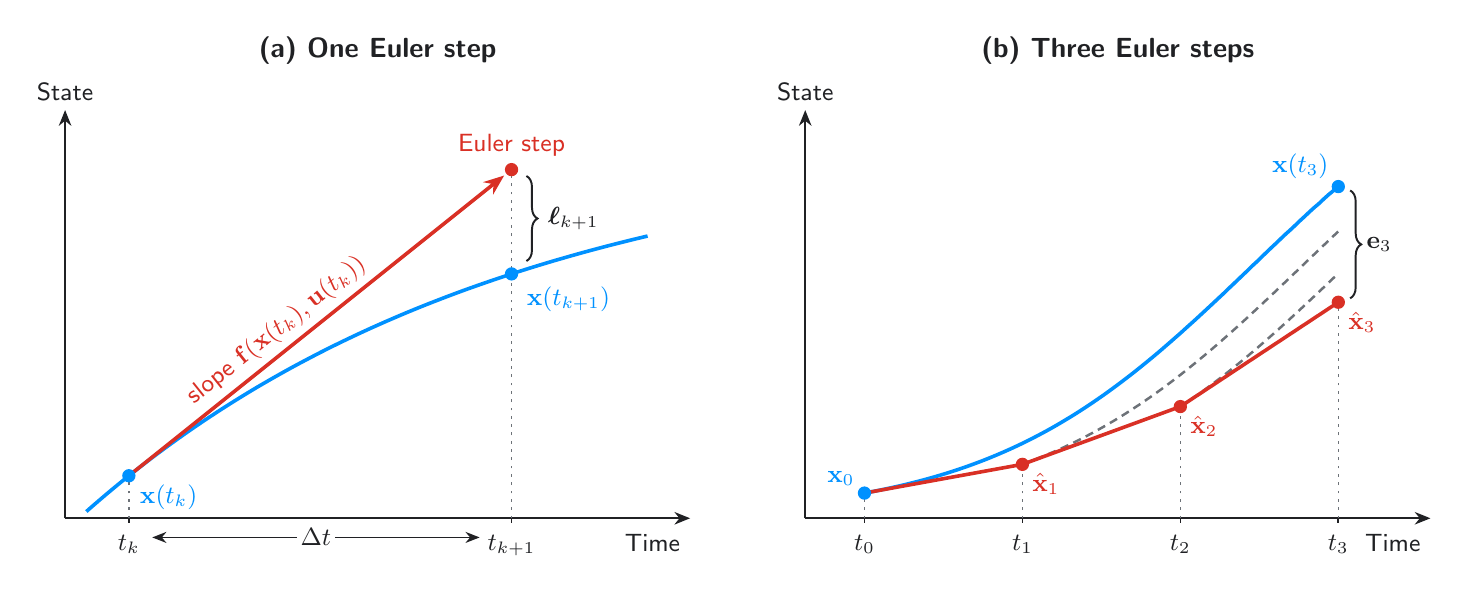
\begin{tikzpicture}

% The two titles share one baseline above the axis boxes.
\node[title] at (3.97, 5.85) {(a) One Euler step};
\node[title] at (13.37, 5.85) {(b) Three Euler steps};

% ------------------------------------------------------------ (a) one step
% The axis corner (-0.15, 0.1) sits at (0, 0).
\begin{scope}[shift={(0.81cm, -0.54cm)}, x=5.4cm, y=5.4cm]
  \draw[axis] (-0.15, 0.1) -- (1.32, 0.1) node[axlab, anchor=north east, yshift=-2pt] {Time};
  \draw[axis] (-0.15, 0.1) -- (-0.15, 1.06) node[axlab, anchor=south] {State};
  \foreach \t/\name in {0/{t_k}, 0.9/{t_{k+1}}} {
    \draw[tick] (\t, 0.1) -- (\t, 0.088);
    \node[ticklab] at (\t, 0.083) {$\name$};
  }
  % the step size runs between the two tick labels, on their row
  \draw[dim] (0.055, 0.055) -- (0.825, 0.055) node[lab, midway, fill=white] {$\Delta t$};
  \draw[guide] (0, 0.1) -- (0, 0.2);
  \draw[guide] (0.9, 0.1) -- (0.9, 0.92);
  % the exact solution and the Euler step along the tangent
  \draw[exact] plot[domain=-0.1:1.22, samples=80, variable=\t] ({\t}, {1 - 0.8*exp(-\t)});
  \draw[eulerstep] (0, 0.2) -- node[redlab, sloped, above, pos=0.42, yshift=1pt] {slope $\mathbf{f}(\vx(t_k),\mathbf{u}(t_k))$} (0.9, 0.92);
  % the points and the local error
  \fill[bluedot] (0, 0.2) circle (2.4pt);
  \fill[bluedot] (0.9, 0.67474) circle (2.4pt);
  \fill[reddot] (0.9, 0.92) circle (2.4pt);
  \node[bluelab, anchor=north west] at (0.015, 0.19) {$\vx(t_k)$};
  \node[bluelab, anchor=north west] at (0.925, 0.655) {$\vx(t_{k+1})$};
  \node[redlab, anchor=south] at (0.9, 0.94) {Euler step};
  \draw[brace] (0.935, 0.905) -- (0.935, 0.705);
  \node[lab, anchor=west] at (0.975, 0.805) {$\boldsymbol{\ell}_{k+1}$};
\end{scope}

% ------------------------------------------------------------ (b) several steps
% The axis corner (-0.45, 0) sits at (9.4, 0); the box matches panel (a).
\begin{scope}[shift={(10.152cm, 0)}, x=1.6716cm, y=6.4cm]
  \draw[axis] (-0.45, 0) -- (4.3, 0) node[axlab, anchor=north east, yshift=-2pt] {Time};
  \draw[axis] (-0.45, 0) -- (-0.45, 0.81) node[axlab, anchor=south] {State};
  \foreach \t/\name in {0/{t_0}, 1.2/{t_1}, 2.4/{t_2}, 3.6/{t_3}} {
    \draw[tick] (\t, 0) -- (\t, -0.0101);
    \node[ticklab] at (\t, -0.0144) {$\name$};
  }
  \draw[guide] (0, 0) -- (0, 0.05);
  \draw[guide] (1.2, 0) -- (1.2, 0.107);
  \draw[guide] (2.4, 0) -- (2.4, 0.22166);
  \draw[guide] (3.6, 0) -- (3.6, 0.42869);
  % the exact solutions through the computed states, then the exact solution
  \draw[neighbor] plot[domain=1.2:3.6, samples=60, variable=\t] ({\t}, {1/(1 + 8.345794*exp(-(\t - 1.2)))});
  \draw[neighbor] plot[domain=2.4:3.6, samples=40, variable=\t] ({\t}, {1/(1 + 3.511389*exp(-(\t - 2.4)))});
  \draw[exact] plot[domain=0:3.6, samples=100, variable=\t] ({\t}, {1/(1 + 19*exp(-\t))});
  % the Euler path
  \draw[eulerpath] (0, 0.05) -- (1.2, 0.107) -- (2.4, 0.22166) -- (3.6, 0.42869);
  \fill[bluedot] (0, 0.05) circle (2.4pt);
  \fill[bluedot] (3.6, 0.65826) circle (2.4pt);
  \foreach \t/\x in {1.2/0.107, 2.4/0.22166, 3.6/0.42869} {
    \fill[reddot] (\t, \x) circle (2.4pt);
  }
  \node[bluelab, anchor=south east] at (-0.04, 0.056) {$\vx_0$};
  \node[redlab, anchor=north west] at (1.24, 0.098) {$\hx_1$};
  \node[redlab, anchor=north west] at (2.44, 0.212) {$\hx_2$};
  \node[redlab, anchor=north west] at (3.64, 0.419) {$\hx_3$};
  \node[bluelab, anchor=south east] at (3.56, 0.664) {$\vx(t_3)$};
  \draw[brace] (3.69, 0.6505) -- (3.69, 0.4365);
  \node[lab, anchor=west] at (3.78, 0.5435) {$\mathbf{e}_3$};
\end{scope}

\end{tikzpicture}
\end{document}
